\section{Use cases diagrams}

\begin{flushleft}
Concernant les Use cases pour cette extension, j'ai dû en rajouter deux.
\end{flushleft}

\begin{flushleft}
\textbf{Comparer les données de consommations}, celui-ci va permettre à l'utilisateur comme son nom l'indique de comparer ses données, cette faculté a déjà été expliquée dans l'introduction.
\end{flushleft}

\begin{flushleft}
\textbf{Envoyer un mail}, quant à celui-ci, il spécifie que si une donnée d'un client est anormalement élevée, alors le serveur enverra un mail pour l'avertir, comme expliqué également dans l'introduction.
\end{flushleft}

\begin{figure}[h]
\centering
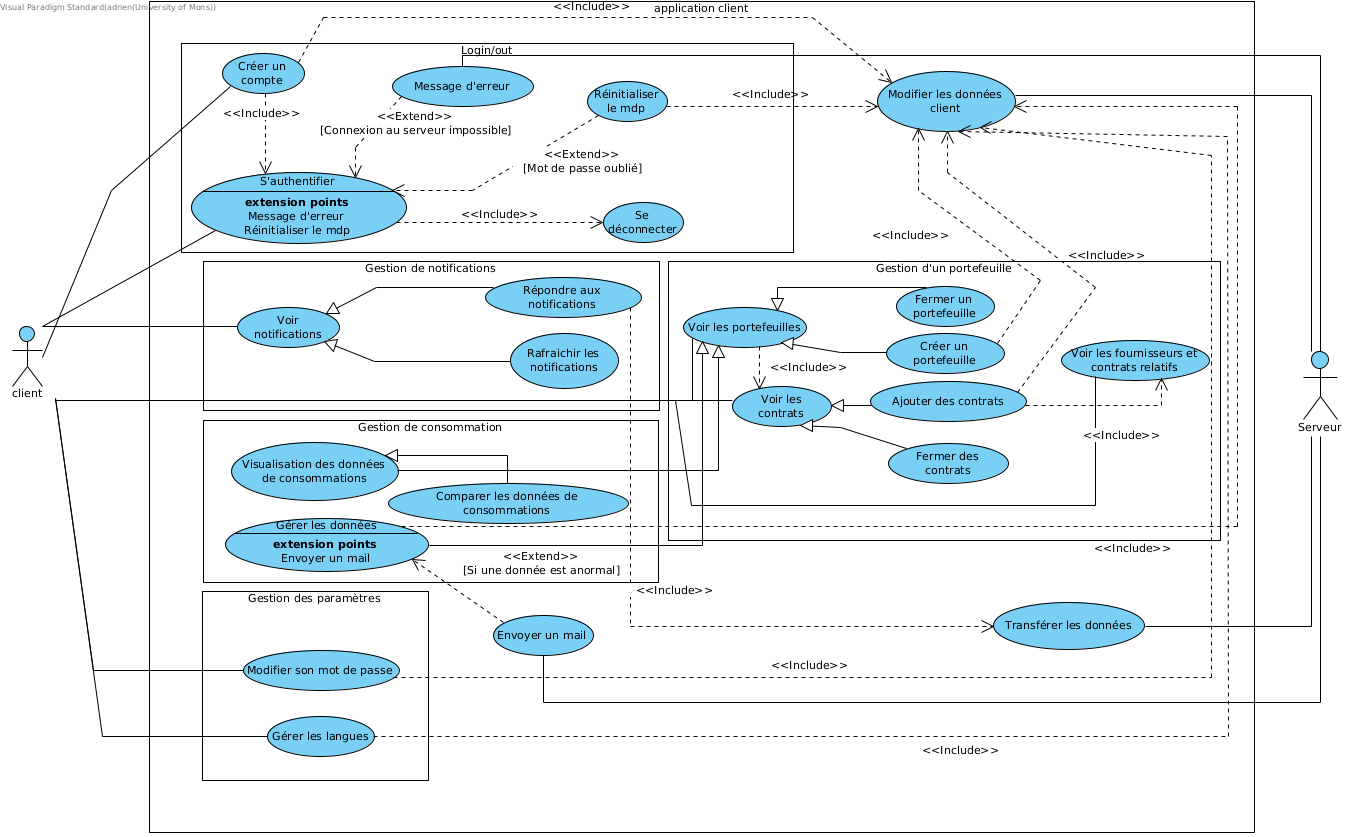
\includegraphics[width=1.3\textwidth]{extension-adrien/Use-case/img/use-case.png}
\end{figure}
